\chapter{Introduction}
\label{chap:introduction}

\section{Background and Motivation}
Vision-Language Models (VLMs) jointly process images and text for tasks such as image captioning, visual question answering, document understanding and instruction following \cite{radford2021learningtransferablevisualmodels,alayrac2022flamingovisuallanguagemodel,li2023blip2bootstrappinglanguageimagepretraining,liu2023visualinstructiontuning,hu2024visualprogramdistillation}.

In this thesis, \textit{multimodal understanding} refers to practical capabilities such as reading text in images, understanding the input question and performing basic reasoning over visual and textual evidence, rather than broad general intelligence.

\begin{figure}[htbp]
    \centering
    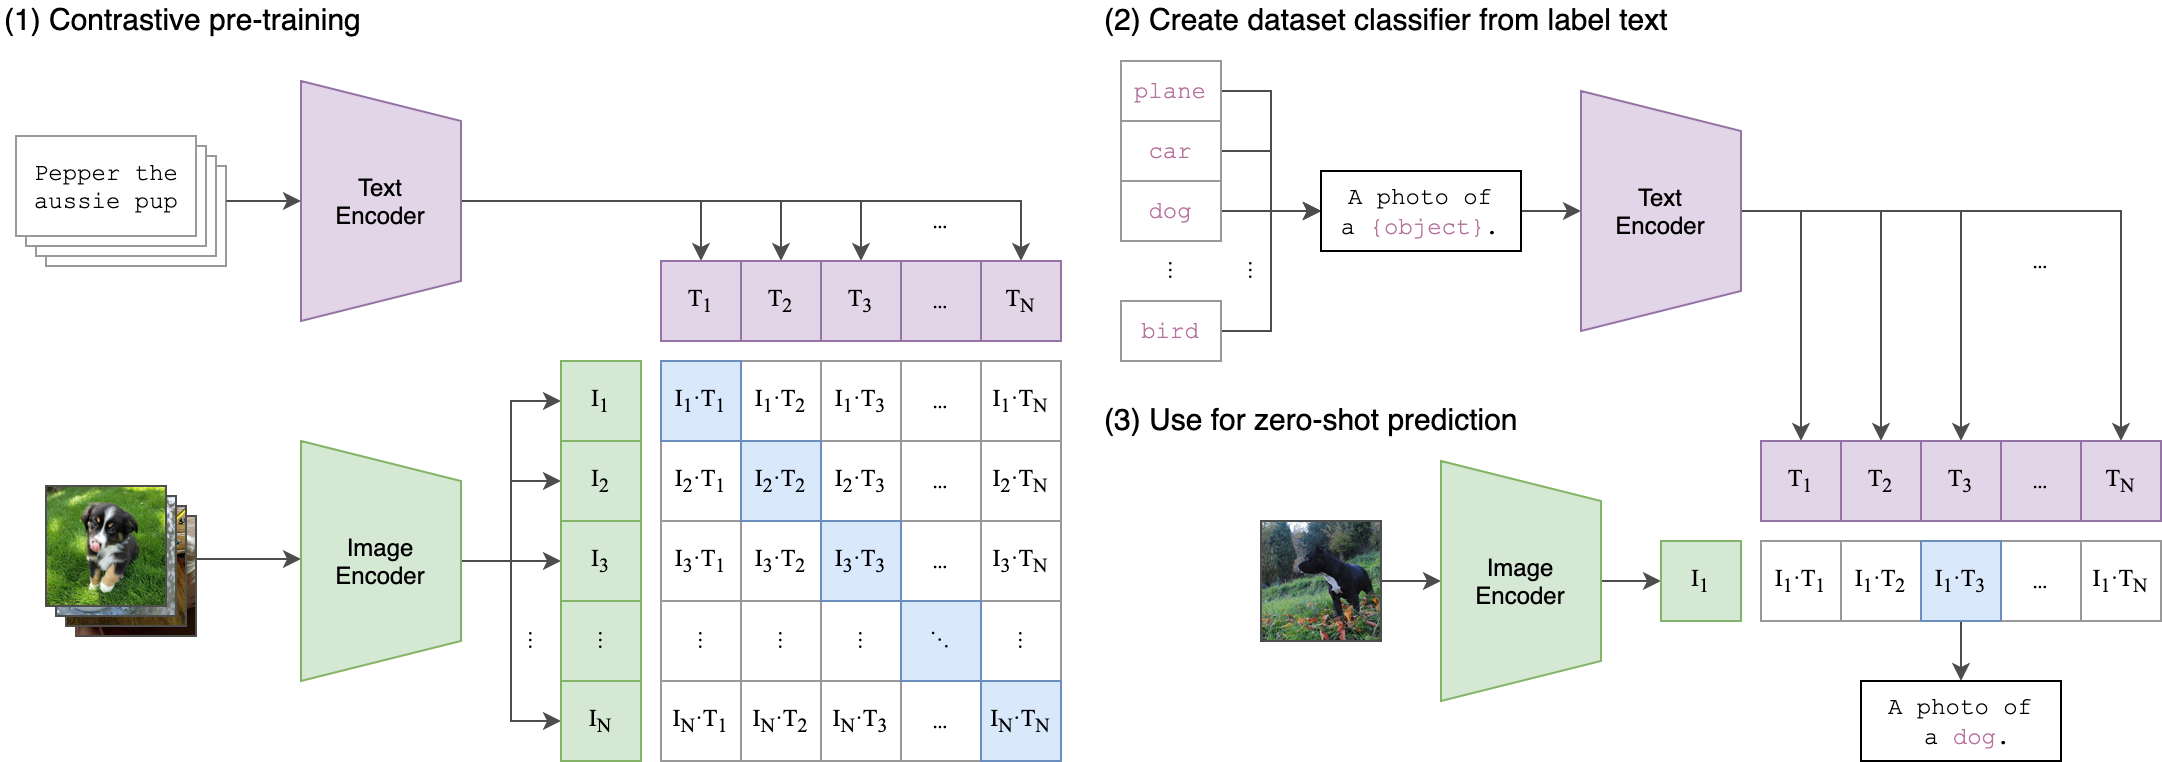
\includegraphics[width=0.82\linewidth]{figures/Contrastive_Language-Image_Pretraining.png}
    \caption{CLIP-style vision-language pretraining aligns image and text representations in a shared embedding space \cite{wikimedia_clip_pretraining_image,radford2021learningtransferablevisualmodels}.}
    \label{fig:intro-vlm-pretraining}
\end{figure}

However, high-performing VLMs are often large and expensive in memory, latency and deployment cost, which limits their use in resource-constrained settings \cite{alayrac2022flamingovisuallanguagemodel,li2023blip2bootstrappinglanguageimagepretraining,chu2023mobilevlm,zhou2024tinyllava}. This issue is especially important for text-centric tasks such as scene-text reading, document understanding and chart reasoning \cite{singh2019vqamodelsread,mathew2021docvqadatasetvqadocument,masry2022chartqabenchmarkquestionanswering}.

\begin{figure}[htbp]
    \centering
    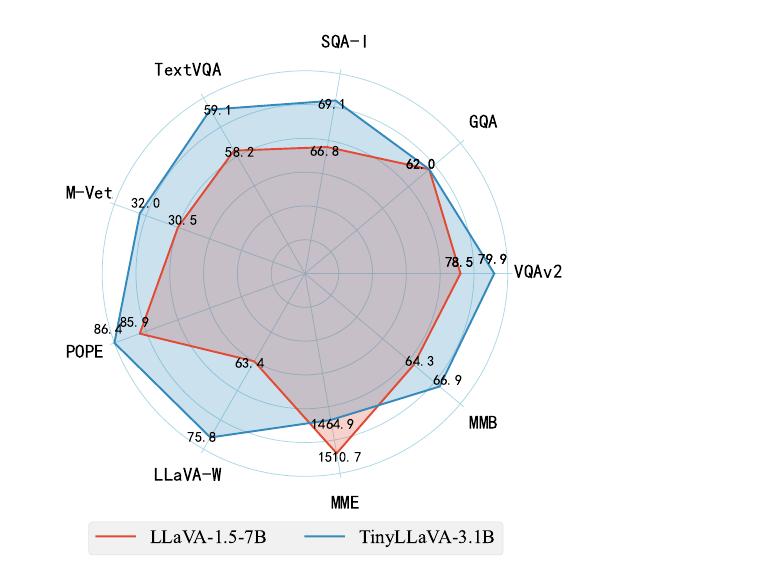
\includegraphics[width=0.66\linewidth]{figures/tinyllava_vs_llava7b_chart.png}
    \caption[TinyLLaVA vs. LLaVA-1.5-7B benchmark comparison.]{Benchmark comparison from TinyLLaVA Figure 1, where a 3.1B small-scale multimodal model remains competitive with the 7B LLaVA-1.5 baseline across several benchmarks \cite{zhou2024tinyllava}.}
    \label{fig:intro-small-vlm-tradeoff}
\end{figure}

Knowledge distillation transfers knowledge from a large teacher to a compact student, achieving competitive performance at lower cost \cite{hinton2015distillingknowledgeneuralnetwork,xu2024surveyknowledgedistillationlarge}. Figure \ref{fig:intro-small-vlm-tradeoff} illustrates why this direction matters: compact multimodal models can remain competitive, but closing the gap to stronger models still requires better transfer of knowledge. In the multimodal setting, recent work has also shown that distillation can be used to transfer reasoning or representation knowledge into more efficient VLMs \cite{hu2024visualprogramdistillation,yang2024clipcid}. For VLMs, this is especially relevant on text-rich benchmarks such as TextVQA, DocVQA and ChartQA \cite{singh2019vqamodelsread,mathew2021docvqadatasetvqadocument,masry2022chartqabenchmarkquestionanswering}.

\begin{figure}[htbp]
    \centering
    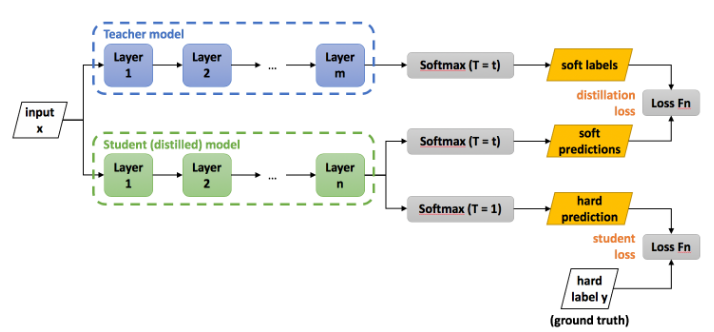
\includegraphics[width=0.70\linewidth]{figures/knowledge_distillation_example.png}
    \caption{Knowledge distillation transfers information from a teacher model to a smaller student model \cite{wikimedia_knowledge_distillation_example,hinton2015distillingknowledgeneuralnetwork}.}
    \label{fig:intro-knowledge-distillation}
\end{figure}

Since no single teacher excels across all multimodal tasks, \textit{multi-teacher distillation} uses multiple complementary teachers with adaptive selection to provide richer, task-relevant supervision \cite{xu2024surveyknowledgedistillationlarge,yuan2020reinforcedmultiteacherselection,zhang2023adaptivemultiteachermetalearning}.

Beyond improving student performance, this thesis also addresses a meta-level problem: \textit{how to choose the right set of teachers for a specific student}. Prior work has shown that fixed or uniform teacher assignment is often suboptimal and recent studies have started to explore adaptive teacher weighting or selective teacher transfer \cite{yuan2020reinforcedmultiteacherselection,zhang2023adaptivemultiteachermetalearning,yu2024selectdistill}. \textbf{To the best of our knowledge, student-specific teacher-set optimization for multimodal VLM distillation remains a completely unexplored problem in the literature.} In this thesis, teacher selection is treated as part of the learning problem itself rather than as a fixed design choice.

This thesis investigates knowledge distillation for VLMs, focusing on how a compact student can learn from multiple teacher VLMs and how teacher-set optimization improves transfer on text-rich multimodal understanding tasks such as reading image text and solving basic reasoning questions in TextVQA, DocVQA and ChartQA \cite{singh2019vqamodelsread,mathew2021docvqadatasetvqadocument,masry2022chartqabenchmarkquestionanswering}.

\section{Problem Statement and Research Objectives}
The central problem addressed in this thesis is how to transfer multimodal understanding ability from large VLMs to compact student models without incurring the full cost of large-scale deployment. In particular, we focus on text-rich multimodal tasks where the student must read image text, understand the question and perform basic reasoning. Existing distillation pipelines usually assume either a single teacher or a fixed set of teachers, which leaves open the harder question of how to select the most useful teachers for a given student model.

Given a pool of \(N\) teacher VLMs and a fixed compact student, the goal is to select \(K\) optimal teachers and train the student to maximize knowledge transfer.

Accordingly, this thesis has three main objectives:
\begin{enumerate}
\item formulate multimodal knowledge distillation for compact VLM students in a text-centric benchmark setting,
\item design an adaptive multi-teacher strategy that treats teacher-set selection as part of the learning problem,
\item evaluate whether teacher-set optimization improves transfer for small VLMs on TextVQA, DocVQA and ChartQA.
\end{enumerate}

\section{Thesis Contributions}
The main contributions of this thesis are summarized as follows:
\begin{enumerate}
\item We formulate student-specific teacher-set optimization for multimodal VLM distillation, focusing on compact students for text-rich multimodal understanding.
\item We propose an adaptive multi-teacher distillation framework in which teacher selection and knowledge transfer are optimized jointly.
\item We study the method on small VLM students and evaluate it on TextVQA, DocVQA and ChartQA using a unified evaluation pipeline.
\end{enumerate}

\section{Thesis Outline}
The remainder of this thesis is organized as follows:
\begin{enumerate}
\item Chapter~\ref{chap:preliminaries} reviews the background on Transformers, VLMs, knowledge distillation and mixture of experts.
\item Chapter~\ref{chap:proposed-method} presents the proposed method, including the problem formulation, teacher selection strategy and training procedure.
\item Chapter~\ref{chap:evaluation-methodology} describes the experimental setup, datasets, evaluation metrics and compared methods.
\item Chapter~\ref{chap:experiment-results} reports the baseline results, comparison results, ablation studies and discussion.
\end{enumerate}
